% Options for packages loaded elsewhere
% Options for packages loaded elsewhere
\PassOptionsToPackage{unicode}{hyperref}
\PassOptionsToPackage{hyphens}{url}
\PassOptionsToPackage{dvipsnames,svgnames,x11names}{xcolor}
%
\documentclass[
  number,
  preprint,
  3p]{elsarticle}
\usepackage{xcolor}
\usepackage{amsmath,amssymb}
\setcounter{secnumdepth}{5}
\usepackage{iftex}
\ifPDFTeX
  \usepackage[T1]{fontenc}
  \usepackage[utf8]{inputenc}
  \usepackage{textcomp} % provide euro and other symbols
\else % if luatex or xetex
  \usepackage{unicode-math} % this also loads fontspec
  \defaultfontfeatures{Scale=MatchLowercase}
  \defaultfontfeatures[\rmfamily]{Ligatures=TeX,Scale=1}
\fi
\usepackage{lmodern}
\ifPDFTeX\else
  % xetex/luatex font selection
\fi
% Use upquote if available, for straight quotes in verbatim environments
\IfFileExists{upquote.sty}{\usepackage{upquote}}{}
\IfFileExists{microtype.sty}{% use microtype if available
  \usepackage[]{microtype}
  \UseMicrotypeSet[protrusion]{basicmath} % disable protrusion for tt fonts
}{}
\makeatletter
\@ifundefined{KOMAClassName}{% if non-KOMA class
  \IfFileExists{parskip.sty}{%
    \usepackage{parskip}
  }{% else
    \setlength{\parindent}{0pt}
    \setlength{\parskip}{6pt plus 2pt minus 1pt}}
}{% if KOMA class
  \KOMAoptions{parskip=half}}
\makeatother
% Make \paragraph and \subparagraph free-standing
\makeatletter
\ifx\paragraph\undefined\else
  \let\oldparagraph\paragraph
  \renewcommand{\paragraph}{
    \@ifstar
      \xxxParagraphStar
      \xxxParagraphNoStar
  }
  \newcommand{\xxxParagraphStar}[1]{\oldparagraph*{#1}\mbox{}}
  \newcommand{\xxxParagraphNoStar}[1]{\oldparagraph{#1}\mbox{}}
\fi
\ifx\subparagraph\undefined\else
  \let\oldsubparagraph\subparagraph
  \renewcommand{\subparagraph}{
    \@ifstar
      \xxxSubParagraphStar
      \xxxSubParagraphNoStar
  }
  \newcommand{\xxxSubParagraphStar}[1]{\oldsubparagraph*{#1}\mbox{}}
  \newcommand{\xxxSubParagraphNoStar}[1]{\oldsubparagraph{#1}\mbox{}}
\fi
\makeatother

\usepackage{color}
\usepackage{fancyvrb}
\newcommand{\VerbBar}{|}
\newcommand{\VERB}{\Verb[commandchars=\\\{\}]}
\DefineVerbatimEnvironment{Highlighting}{Verbatim}{commandchars=\\\{\}}
% Add ',fontsize=\small' for more characters per line
\usepackage{framed}
\definecolor{shadecolor}{RGB}{241,243,245}
\newenvironment{Shaded}{\begin{snugshade}}{\end{snugshade}}
\newcommand{\AlertTok}[1]{\textcolor[rgb]{0.68,0.00,0.00}{#1}}
\newcommand{\AnnotationTok}[1]{\textcolor[rgb]{0.37,0.37,0.37}{#1}}
\newcommand{\AttributeTok}[1]{\textcolor[rgb]{0.40,0.45,0.13}{#1}}
\newcommand{\BaseNTok}[1]{\textcolor[rgb]{0.68,0.00,0.00}{#1}}
\newcommand{\BuiltInTok}[1]{\textcolor[rgb]{0.00,0.23,0.31}{#1}}
\newcommand{\CharTok}[1]{\textcolor[rgb]{0.13,0.47,0.30}{#1}}
\newcommand{\CommentTok}[1]{\textcolor[rgb]{0.37,0.37,0.37}{#1}}
\newcommand{\CommentVarTok}[1]{\textcolor[rgb]{0.37,0.37,0.37}{\textit{#1}}}
\newcommand{\ConstantTok}[1]{\textcolor[rgb]{0.56,0.35,0.01}{#1}}
\newcommand{\ControlFlowTok}[1]{\textcolor[rgb]{0.00,0.23,0.31}{\textbf{#1}}}
\newcommand{\DataTypeTok}[1]{\textcolor[rgb]{0.68,0.00,0.00}{#1}}
\newcommand{\DecValTok}[1]{\textcolor[rgb]{0.68,0.00,0.00}{#1}}
\newcommand{\DocumentationTok}[1]{\textcolor[rgb]{0.37,0.37,0.37}{\textit{#1}}}
\newcommand{\ErrorTok}[1]{\textcolor[rgb]{0.68,0.00,0.00}{#1}}
\newcommand{\ExtensionTok}[1]{\textcolor[rgb]{0.00,0.23,0.31}{#1}}
\newcommand{\FloatTok}[1]{\textcolor[rgb]{0.68,0.00,0.00}{#1}}
\newcommand{\FunctionTok}[1]{\textcolor[rgb]{0.28,0.35,0.67}{#1}}
\newcommand{\ImportTok}[1]{\textcolor[rgb]{0.00,0.46,0.62}{#1}}
\newcommand{\InformationTok}[1]{\textcolor[rgb]{0.37,0.37,0.37}{#1}}
\newcommand{\KeywordTok}[1]{\textcolor[rgb]{0.00,0.23,0.31}{\textbf{#1}}}
\newcommand{\NormalTok}[1]{\textcolor[rgb]{0.00,0.23,0.31}{#1}}
\newcommand{\OperatorTok}[1]{\textcolor[rgb]{0.37,0.37,0.37}{#1}}
\newcommand{\OtherTok}[1]{\textcolor[rgb]{0.00,0.23,0.31}{#1}}
\newcommand{\PreprocessorTok}[1]{\textcolor[rgb]{0.68,0.00,0.00}{#1}}
\newcommand{\RegionMarkerTok}[1]{\textcolor[rgb]{0.00,0.23,0.31}{#1}}
\newcommand{\SpecialCharTok}[1]{\textcolor[rgb]{0.37,0.37,0.37}{#1}}
\newcommand{\SpecialStringTok}[1]{\textcolor[rgb]{0.13,0.47,0.30}{#1}}
\newcommand{\StringTok}[1]{\textcolor[rgb]{0.13,0.47,0.30}{#1}}
\newcommand{\VariableTok}[1]{\textcolor[rgb]{0.07,0.07,0.07}{#1}}
\newcommand{\VerbatimStringTok}[1]{\textcolor[rgb]{0.13,0.47,0.30}{#1}}
\newcommand{\WarningTok}[1]{\textcolor[rgb]{0.37,0.37,0.37}{\textit{#1}}}

\usepackage{longtable,booktabs,array}
\newcounter{none} % for unnumbered tables
\usepackage{calc} % for calculating minipage widths
% Correct order of tables after \paragraph or \subparagraph
\usepackage{etoolbox}
\makeatletter
\patchcmd\longtable{\par}{\if@noskipsec\mbox{}\fi\par}{}{}
\makeatother
% Allow footnotes in longtable head/foot
\IfFileExists{footnotehyper.sty}{\usepackage{footnotehyper}}{\usepackage{footnote}}
\makesavenoteenv{longtable}
\usepackage{graphicx}
\makeatletter
\newsavebox\pandoc@box
\newcommand*\pandocbounded[1]{% scales image to fit in text height/width
  \sbox\pandoc@box{#1}%
  \Gscale@div\@tempa{\textheight}{\dimexpr\ht\pandoc@box+\dp\pandoc@box\relax}%
  \Gscale@div\@tempb{\linewidth}{\wd\pandoc@box}%
  \ifdim\@tempb\p@<\@tempa\p@\let\@tempa\@tempb\fi% select the smaller of both
  \ifdim\@tempa\p@<\p@\scalebox{\@tempa}{\usebox\pandoc@box}%
  \else\usebox{\pandoc@box}%
  \fi%
}
% Set default figure placement to htbp
\def\fps@figure{htbp}
\makeatother





\setlength{\emergencystretch}{3em} % prevent overfull lines

\providecommand{\tightlist}{%
  \setlength{\itemsep}{0pt}\setlength{\parskip}{0pt}}



 
\usepackage[]{natbib}
\bibliographystyle{elsarticle-num}


\makeatletter
\@ifpackageloaded{caption}{}{\usepackage{caption}}
\AtBeginDocument{%
\ifdefined\contentsname
  \renewcommand*\contentsname{Table of contents}
\else
  \newcommand\contentsname{Table of contents}
\fi
\ifdefined\listfigurename
  \renewcommand*\listfigurename{List of Figures}
\else
  \newcommand\listfigurename{List of Figures}
\fi
\ifdefined\listtablename
  \renewcommand*\listtablename{List of Tables}
\else
  \newcommand\listtablename{List of Tables}
\fi
\ifdefined\figurename
  \renewcommand*\figurename{Figure}
\else
  \newcommand\figurename{Figure}
\fi
\ifdefined\tablename
  \renewcommand*\tablename{Table}
\else
  \newcommand\tablename{Table}
\fi
}
\@ifpackageloaded{float}{}{\usepackage{float}}
\floatstyle{ruled}
\@ifundefined{c@chapter}{\newfloat{codelisting}{h}{lop}}{\newfloat{codelisting}{h}{lop}[chapter]}
\floatname{codelisting}{Listing}
\newcommand*\listoflistings{\listof{codelisting}{List of Listings}}
\makeatother
\makeatletter
\makeatother
\makeatletter
\@ifpackageloaded{caption}{}{\usepackage{caption}}
\@ifpackageloaded{subcaption}{}{\usepackage{subcaption}}
\makeatother
\usepackage{bookmark}
\IfFileExists{xurl.sty}{\usepackage{xurl}}{} % add URL line breaks if available
\urlstyle{same}
% fallback for those not using the hyperref driver hyperxmp:
\makeatletter
\@ifundefined{xmpquote}{\newcommand{\xmpquote}[1]{#1}}{}
\makeatother
\hypersetup{
  pdftitle={Echolabel: Image-based echogram annotation tool for aquatic ecology},
  pdfauthor={Gaspard Ringuenet; Alejandro Ariza; Gildas Roudaut; William Puech; Arnaud Bertrand},
  pdfkeywords={\xmpquote{Active
acoustics}, \xmpquote{Multifrequency}, \xmpquote{Echogram
annotation}, \xmpquote{Aquatic ecology}, \xmpquote{Open source}},
  colorlinks=true,
  linkcolor={blue},
  filecolor={Maroon},
  citecolor={Blue},
  urlcolor={Blue},
  pdfcreator={LaTeX via pandoc}}


\setlength{\parindent}{6pt}
\begin{document}

\begin{frontmatter}
\title{Echolabel: Image-based echogram annotation tool for aquatic
ecology}
\author[1]{Gaspard Ringuenet%
\corref{cor1}%
}
 \ead{gaspard.ringuenet@umontpellier.fr} 
\author[2]{Alejandro Ariza%
%
}
 \ead{alejandro.ariza@ifremer.fr} 
\author[3]{Gildas Roudaut%
%
}
 \ead{gildas.roudaut@ird.fr} 
\author[4]{William Puech%
%
}
 \ead{william.puech@lirmm.fr} 
\author[1]{Arnaud Bertrand%
%
}
 \ead{arnaud.bertrand@ird.fr} 

\affiliation[1]{organization={MARBEC, Université de Montpellier, CNRS,
Ifremer, IRD, Montpellier, France},,postcodesep={}}
\affiliation[2]{organization={DECOD, Ifremer, INRAE, Institut Agro,
Nantes, France},,postcodesep={}}
\affiliation[3]{organization={LEMAR, UBO, IFREMER, IRD, CNRS, Technopole
Brest Iroise, Plouzané, France},,postcodesep={}}
\affiliation[4]{organization={LIRMM, Université de Montpellier, CNRS,
Montpellier, France},,postcodesep={}}

\cortext[cor1]{Corresponding author}





        
\begin{abstract}
Active acoustic systems are essential for studying aquatic ecosystems,
delivering high-resolution information over large spatial scales. Yet
processing these data still relies heavily on manual annotation, and to
the best of our knowledge, no open-source software currently exists for
this task. We present Echolabel, an open-source, cross-platform tool for
fast echogram visualization and annotation, which produces CSV outputs
directly compatible with Echoregions, an annotation handling package
within Echostack, the emerging Python toolkit for echosounder data.
Echolabel is deliberately minimal and task-specific, and is not intended
to substitute for a general-purpose acoustic processing software. The
tool is available as a command-line interface and as a Python
application programming interface. It builds on the LabelMe graphical
user interface to annotate cached echogram images and transparently
converts between images and physical (time, depth) coordinates.
Visualization options include RGB-composite echograms, which combine
several acoustic frequencies and enable annotations informed by the
frequency response of the imaged targets. We demonstrate the practical
utility of Echolabel, combined with Echoregions, on routine annotation
tasks and a brief ecological analysis. Echolabel is particularly well
suited to delineating irregular, fuzzy objects such as sound-scattering
layers, and thus facilitates the sonar-based investigation of aquatic
ecosystems.
\end{abstract}





\begin{keyword}
    Active acoustics \sep Multifrequency \sep Echogram
annotation \sep Aquatic ecology \sep 
    Open source
\end{keyword}
\end{frontmatter}
    

\section*{Metadata}\label{metadata}
\addcontentsline{toc}{section}{Metadata}

{\def\LTcaptype{none} % do not increment counter
\begin{longtable}[]{@{}
  >{\raggedright\arraybackslash}p{(\linewidth - 4\tabcolsep) * \real{0.1000}}
  >{\raggedright\arraybackslash}p{(\linewidth - 4\tabcolsep) * \real{0.3000}}
  >{\raggedright\arraybackslash}p{(\linewidth - 4\tabcolsep) * \real{0.6000}}@{}}
\toprule\noalign{}
\begin{minipage}[b]{\linewidth}\raggedright
Nr
\end{minipage} & \begin{minipage}[b]{\linewidth}\raggedright
Code metadata description
\end{minipage} & \begin{minipage}[b]{\linewidth}\raggedright
Metadata
\end{minipage} \\
\midrule\noalign{}
\endhead
\bottomrule\noalign{}
\endlastfoot
C1 & Current code version & V0.1.0 \\
C2 & Permanent link to code/repository used for this code version &
\url{https://github.com/gaspardringuenet/echolabel} \\
C3 & Permanent link to reproducible capsule & \\
C4 & Legal code license & GPL-3.0 license \\
C5 & Code versioning system used & Git \\
C6 & Software code languages, tools and services used & Python \\
C7 & Compilation requirements, operating environments and dependencies &
Requires Python \(\geq\) 3.12 \\
C8 & If available, link to developer documentation/manual &
\url{https://github.com/gaspardringuenet/echolabel/README.md} \\
C9 & Support email for questions &
\href{mailto:gaspard.ringuenet@umontpellier.fr}{\nolinkurl{gaspard.ringuenet@umontpellier.fr}} \\
\end{longtable}
}

\section{Motivation and Significance}\label{motivation-and-significance}

Aquatic ecosystems, from lakes and rivers to coastal waters and the open
ocean, are largely hidden from direct observation. Many of their
organisms live in the water column, which direct sampling with nets or
traps covers only sparsely, at high cost and often invasively. In this
context, active acoustic systems (sonars) provide crucial information:
by sounding the water column at high resolution, they are the only
technology capable of providing continuous observations of organism
distribution and behavior at the spatial and temporal scales at which
physical and ecological processes occur \citep{benoit-bird2016}.

Although the tool presented in this paper applies to echograms from any
aquatic environment, the examples come from the pelagic ocean. The
pelagic zone designates the water column away from the seabed. This vast
three-dimensional habitat represents more than 90 \% of the available
living volume on the planet. Lacking hard physical structures in
comparison to the benthic zone (i.e., the seabed) or land, it can be
divided into depth layers based on light penetration. The mesopelagic,
where less than 1 \% of light reaches, typically spans from 200 m to
1000 m. Its significance is evident from its large biomass and diversity
\citep{irigoien2014, eduardo2024, haddock2024}, its crucial role in
ocean functioning \citep{robinson2010, passow2012}, and its
interdependence with human societies \citep{martin2020, eduardo2025}.
Despite this, the ``twilight zone'' remains understudied, primarily due
to technical limitations in investigating deep waters. Active acoustics
is particularly valuable here, as echosounders can sample the water
column up to \textasciitilde1000 m with high resolution.

However, extracting ecological information from acoustic data remains a
major challenge. Manual delineation of features in echograms has long
been a common practice in marine acoustics. Targeted biological features
are most often aggregations such as fish schools or krill swarms, but
may also include sound-scattering layers, which comprise a wide variety
of organisms, from invertebrates to fish, distributed horizontally in
the water column.

Annotating these features is part of the daily routine in ecosystem
acoustic surveys, whether for subsequent analyses of distribution and
biomass or to populate libraries used to train machine learning models
for species identification. Several software solutions are currently
available for this purpose: commercial options such as Echoview
\citep{echoview}; free but closed-source Windows-based software such as
LSSS\footnote{LSSS now has an open-source version, and it is available
  for linux and macOs (\url{https://marec.no/downloads.htm}).}
\citep{korneliussen2006} and Movies3D \citep{trenkel2009}; or
open-source software requiring a proprietary MATLAB license, such as
ESP3 and Matecho \citep{ladroit2020, perrot2018}.

In recent years, there has been significant development of free,
open-source, cross-platform software for ecosystem acoustics. The most
notable example, both in terms of development and engagement from the
scientific community, is Echostack, a suite of Python packages for
performing various routine tasks with scientific echosounder data
\citep{lee2024, lee2024a}. Echostack includes the
\href{https://github.com/OSOceanAcoustics/echoregions}{Echoregions}
package, designed to parse acoustic annotations and interface them with
the gridded acoustic data. The package contains functions to create
masks for machine learning models training or for routine processing
tasks such as biomass estimation. However, no open-source solution is
available for such annotations yet, despite this being one of the tasks
that acoustic operators spend the most time on, and the first step in
ecosystem acoustic processing.

To bridge this gap, we propose Echolabel, a minimalist Python
application for echogram annotation, built to be interoperable with
Echostack / Echoregions. Its scope is narrower than that of most
GUI-based acoustic software, which provide suites of analysis-ready
computation tools. Echolabel rather focuses on the annotation task only,
and is thought as a module in open-source acoustic processing pipelines.
To do so it leverages the power of LabelMe \citep{kentaro}, a widely
used open-source Python application for image annotation, by converting
acoustic data into a set of echogram images. The output is an
Echoregions-compatible CSV file, ensuring integration into the Python
acoustic data processing environment. Echolabel is free, open-source,
cross-platform, and free of proprietary dependencies. It requires little
computing power, and offers an easy-to-use GUI for annotation

\section{Software description}\label{software-description}

\subsection{Software architecture}\label{software-architecture}

The software is written in Python, with separate modules responsible for
application configuration, command-line inputs, cached data management,
and parsing annotation files.

It is minimalist, comprising 13 Python modules with rougly 100 - 200
lines of code each, and avoids re-implementing existing functionalities
as much as possible. The annotation interface is entirely provided by
LabelMe v6.0.0 \citep{kentaro2}, and Echolabel focuses on parsing
annotations between LabelMe and Echoregions. The annotation parsing
module is called \texttt{regions2d\_extension} and mimics Echoregions'
code to parse Echoview annotation data, with the aim of providing clear
insight into the application's purpose.

Echolabel has been developed to be primarily used from the command-line
interface (CLI; see Listing~\ref{lst-escore-demo}). The main
\texttt{process} command triggers conversion of the acoustic data into
images before automatically running LabelMe. It features a number of
optional parameters, allowing the user to modify the echogram. Passed
CLI parameters are used to override a default configuration file, which
can be directly edited for improved control and reproducibility. If
necessary, a programming interface remains available with the
\texttt{EcholabelApp} and \texttt{Config} classes at the top level.

A series of unit tests ensure that core features are preserved across
future updates. Tested functionalities include configuration, data
loading, image-dataset management, and annotation parsing. Git is used
for version control.

\subsection{Software functionalities}\label{software-functionalities}

Echolabel wrapps around LabelMe, essentially handling shapes coordinates
conversion logic. It loads acoustic data, chunks it into a dataset of
echogram images, and runs LabelMe. When the user exits the LabelMe GUI,
the image-based annotations are converted to physical (time, depth)
coordinates and saved in a format that can be read using Echoregions.

Echolabel works with processed, gridded volume backscattering strength
data (Sv, dB) \citep{maclennan2002}, i.e., the widely used acoustic
measure for characterizing the distribution of organisms in the water
column, after the data have been cleaned of artifacts and regridded onto
a consistent grid across frequency, depth, and time--distance
dimensions. By default, Echolabel supports two widely used conventions
for distributing data with this structure and level of processing: the
IMOS SOOP-BA NetCDF data format \citep{kunnath2018} and the
coordinate/variable names adopted by Echostack (namely using
``ping\_time'' instead of ``time'' as time dimension coordinate name).
For full flexibility, it can support any variable names, provided that
the user manually identifies Sv, depth, and time--distance variables in
the configuration file. Both NetCDF files and Zarr stores are accepted
as input formats. Several files in the same directory may be loaded as a
single dataset as long as their coordinates are compatible.

Common echogram visualization options are provided. Indeed, the user can
select the visualized frequency and specify value bounds as well as the
colormap. A wide range of matplotlib colormaps can be selected using
their names. In addition to single-frequency echograms, Echolabel offers
a triple-frequency RGB echogram mode in which three channels are mapped
to each of the red, green, and blue channels (with equal bounds). This
visualization method is very effective for assessing the distribution of
frequency responses across the echogram (for examples see
\citep{ariza2022, annasawmy2019}). The background (where no channel is
active) colour can also be specified in the configuration (as a
matplotlib-compatible string or tuple).

Running the application triggers data loading and the building and
caching of an echogram image dataset using visualization options.
Echogram images are the representation of acoustic data once colour
mapping has been applied. Each pixel represents a sampled volume. Each
image's physical (time and depth) coordinates are saved in cache. The
image dataset building step is the only step involving significant
computation. While lazy-loading of the acoustic dataset prevents memory
overload, this step may take up to a few minutes for large-scale surveys
with high resolution data. To avoid rebuilding the images at each
session, Echolabel enables reuse of the cached images, allowing the GUI
to launch almost instantaneously.

A prominent feature of Echolabel is the LabelMe graphical user interface
(GUI; Figure~\ref{fig-demo-gui}), which is used to create annotations.
This relies on the prior conversion of the acoustic data into images.
Within the open window, the user can loop through the images in the
``File List'' panel. They can also visualize and edit existing
annotations using the ``Annotation List'' panel and point clicks. Most
importantly, they can use the ``CreateShapeTools'' to add new shapes.
All changes are automatically saved in cache as LabelMe JSON annotations
during the GUI editing session. The GUI is customizable, and the user
has the option to edit the LabelMe configuration file on their system.
Since Echolabel runs LabelMe as a subprocess and only operates on
annotation files, modifying the LabelMe configuration should not create
conflicts.

When closing the GUI, shape annotations are parsed and saved as a CSV
file compatible with the
\href{https://github.com/echostack-org/echoregions/blob/main/echoregions/regions2d/regions2d.py}{\texttt{echoregions.Regions2D}}
class. This conversion uses the saved image coordinates to convert
pixel-wise annotations into (time, depth) points. \texttt{Regions2D}
objects can represent polygons only. For this reason, polygon and
rectangle LabelMe tools are the only ones whose shapes can be converted
(output from other tools is ignored). Once the annotation-format
conversion is done, the CSV file is created or updated, and is then
ready to be loaded into Echoregions in a single line.

Additional features include a \texttt{demo} command that downloads and
processes demonstration data. It is also worth noting that LabelMe
provides an AI polygon creation tool. The tool installs an image
segmentation model (Meta's Segment Anything Model 2 as of LabelMe
v6.0.0) locally to provide assistance by automatically delineating
objects. While such models are efficient on natural images, they appear
much less useful on echograms. However, since the tool produces
polygons, annotations are correctly parsed by Echolabel.

\section{Illustrative examples}\label{illustrative-examples}

\subsection{Polygon annotation on RGB
echogram}\label{polygon-annotation-on-rgb-echogram}

The ABRAÇOS II survey was conducted off the north-eastern coast of
Brazil during the Austral fall of 2017 (April 9\textsuperscript{th} --
May 7\textsuperscript{th}). Research vessel Antea of the French
oceanographic fleet operated a hull-mounted EK60 echosounder at four
frequencies (38, 70, 120, and 200 kHz) with a pulse length of 512 μs
\citep{abracos2cruise, bertrand2026}. Two configurations were used: a
ping rate of 0.45 s for seabed depth less than 150 m, and a ping rate of
2.4 s for deeper areas, recording to depth up to 750 m. The echosounder
was calibrated mid-survey in Fernando de Noronha using standard
protocols \citep{demer2015}. Acoustic data processing was conducted
using the Matecho software. Noise and artifact removal was performed
using a combination of automated and manual cleaning tools. Volume
backscattering strength was echo-integrated with a minimum threshold of
-90 dB in 3-pings by 1-m cells. A conversion from the MATLAB format used
by Matecho to a Zarr store was applied to the echo-integrated product.
The demonstration data used thereafter are a 10-hour subset of the
ABRAÇOS II survey, spanning both open ocean and part of the shelf of the
Fernando de Noronha island up to \textasciitilde50 m deep.

Several objects of interest are selected from the demonstration dataset
using Echolabel. The GUI is launched from the terminal using a simple
command, rendering an RGB composite echogram showing 38, 70, and 120 kHz
channels simultaneously (Listing~\ref{lst-escore-demo}). Selected
features are delineated using the ``Create Polygons'' and ``Create
Rectangles'' tools and assigned text labels (Figure~\ref{fig-demo-gui}):
a sound-scattering layer (``Layer''), a probable fish aggregation
(``School''), a v-shaped anomaly probably caused by a lowered instrument
(``Artifact''), and rectangle areas of varying hue (``Unknown''). The
eight annotated regions are saved as a CSV file when closing the
graphical interface.

\begin{codelisting}

\caption{\label{lst-escore-demo}Example bash command to build an RGB
echogram and run the ROI demonstration.}

\centering{

\begin{Shaded}
\begin{Highlighting}[]
\ExtensionTok{echolabel}\NormalTok{ process }\DataTypeTok{\textbackslash{}}
\NormalTok{{-}s data/demo.zarr }\DataTypeTok{\textbackslash{} }                \CommentTok{\# acoustic data store}
\ExtensionTok{{-}o}\NormalTok{ data/demo\_regions.csv }\DataTypeTok{\textbackslash{} }         \CommentTok{\# annotation file}
\ExtensionTok{{-}f}\NormalTok{ 38000 }\AttributeTok{{-}f}\NormalTok{ 70000 }\AttributeTok{{-}f}\NormalTok{ 120000 }\DataTypeTok{\textbackslash{} }      \CommentTok{\# mapped frequencies (Hz)}
\ExtensionTok{{-}{-}cmap}\NormalTok{ RGB }\DataTypeTok{\textbackslash{} }                       \CommentTok{\# RGB composite echogram}
\ExtensionTok{{-}{-}vmin} \AttributeTok{{-}90} \AttributeTok{{-}{-}vmax} \AttributeTok{{-}50}               \CommentTok{\# Color scale bounds}
\end{Highlighting}
\end{Shaded}

}

\end{codelisting}%

\begin{figure}

\centering{

\pandocbounded{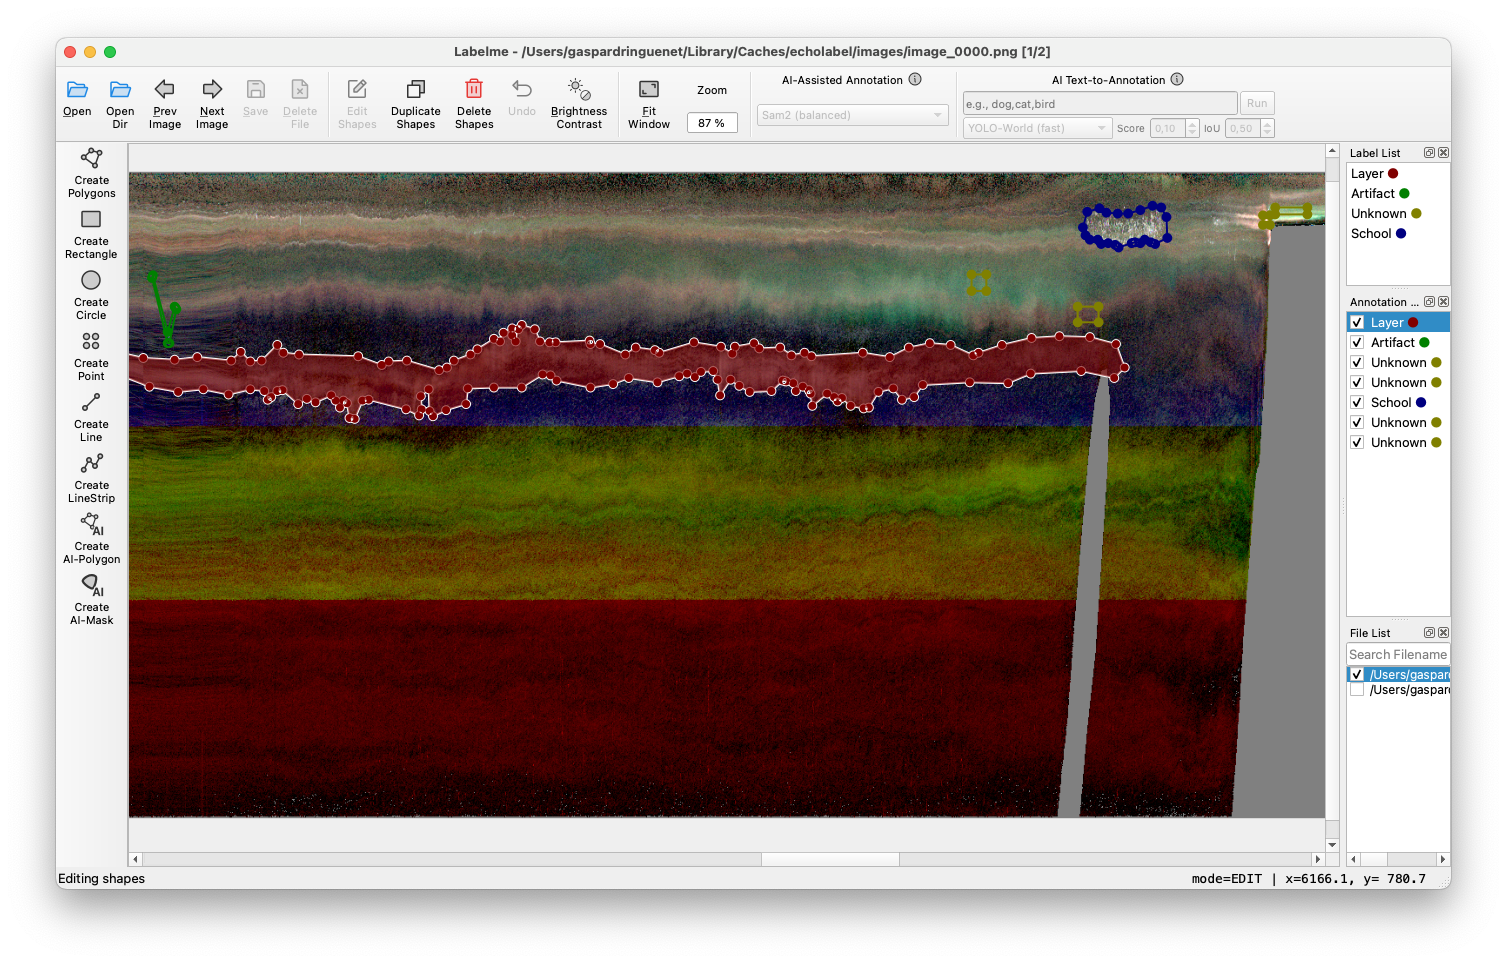
\includegraphics[keepaspectratio]{images/region_selection.png}}

}

\caption{\label{fig-demo-gui}LabelMe graphical user interface showing
drawn regions on an RGB composite echogram (R: 38 kHz; G: 70 kHz; B: 120
kHz - as specified in Listing~\ref{lst-escore-demo}) in the image panel
(center). The elongated grey shape is masked out double echo data. The
second grey shape on the right of the echogram indicates pixels below
the ocean floor. Horizontal colour boundaries result from the channels'
range limits (e.g.~the 120 kHz channel becomes to noisy around 250 m
deep and data is removed below). Manually created polygonal shapes are
overlayed on top of the echogram. The associated labels with are visible
in the ``Annotation List'' panel, and as a non-duplicated list in the
``Label List'' panel. A ``Layer'' annotation and the corresponding
polygon are being edited and so they are highlighted. The ``File List''
panel shows all available echogram images.}

\end{figure}%

Echolabel solely focuses on creating the annotations, but the software's
strength lies in its immediate compatibility with the Echoregions
package. The following sections therefore demonstrate first-order use
cases for such annotations using Echoregions.

\subsection{Use case 1 - Routine
tasks}\label{use-case-1---routine-tasks}

Figure~\ref{fig-basic-tasks} shows regions with the ``Unknown'',
``Artifact'', and ``School'' labels (a), along with processing or data
analysis steps corresponding to the underlying echogram features (b-g):
frequency response investigation, artifact removal, and aggregation mask
extraction, respectively. All of those are made possible by the masking
functionality of Echoregions (using the
\href{https://regionmask.readthedocs.io}{regionmask} package) package)
and each requires no more than a dozen lines of code to compute
(omitting figure building).

The most basic task is computing the frequency responses of an echogram
region. The influence of the organisms' anatomy on their back-scattering
properties has long been acknowledged, and is the motivation for
multifrequency acoustics \citep{benoit-bird2016}. Spatio-temporal
variations in frequency responses can then be attributed to variations
in the species (or age) composition in the sampled volumes. While the
RGB echogram successfully renders part of this contrast, a quantitative
comparison of back-scattering between regions of interest provides a
more exhaustive and objective insight. Figure~\ref{fig-basic-tasks} b,c
compares two reddish (38 kHz dominant) and two greenish (70 kHz
dominant) regions, in different oceanographic setups (pelagic or on
shelf edge), depths (150 m or 50 m) and intensity (seemingly stronger
near the shelf) by computing the frequency response relative to the 38
kHz channel
(\(R(f) = \Delta \text{MVBS}_{f - 38 \text{kHz}} = S_{v}(f) - S_{v}(38 \text{ kHz})\)
; see \citep{maclennan2002} for notation) for all regions. Green regions
contain similar R(f). On the other hand, red regions show great
differences, especially at 120 and 200 kHz, suggesting a very different
biological composition. Further analysis using this kind of regions of
interest may include target strength (TS) modelling, or building a
training set for a multifrequency classification algorithm.

Despite a thorough cleaning of acoustic data, some unwanted signal or
noise may still be present in the final product. This is accentuated by
the context-dependence of unwanted signal. Manual cleaning of the
echo-integrated product can easily be conducted with the combination of
Echolabel and Echoregions. This is demonstrated in
Figure~\ref{fig-basic-tasks} d,e in which the back-scattering of a
probable CTD profiler is removed using a polygonal shape.

On the contrary, one may want to extract the mask of a biological
aggregation of interest. This is common for fish schools and shoals, and
illustrated in Figure~\ref{fig-basic-tasks} f,g. A typical use of such
masks is supervised deep learning model training. Computation of
acoustic variables, or post processing of the mask (for instance to
remove unwanted pixels) may also apply to fish aggregations.

\begin{figure}

\centering{

\pandocbounded{\includegraphics[keepaspectratio]{index_files/mediabag/images/basic-annotation-tasks-wlayer.pdf}}

}

\caption{\label{fig-basic-tasks}Annotated echogram regions and simple
use cases. (a) Annotated polygonal regions displayed on top of an RGB
echogram, with the dashed line representing the ``Layer'' polygon. (b-g)
Use cases: the annotated rectangles (b) can be used to compute the mean
and standard deviation of relative frequency responses of data within
(c); a v-shaped anomaly, typical of a lowered instrument (d) can be
masked out (e); the binary mask (g) of a fish aggregation (f) can be
computed.}

\end{figure}%

\subsection{Use case 2 - Analysis of a sound-scattering
layer}\label{use-case-2---analysis-of-a-sound-scattering-layer}

\begin{figure}

\centering{

\pandocbounded{\includegraphics[keepaspectratio]{index_files/mediabag/images/fuzzy-layer-analysis.pdf}}

}

\caption{\label{fig-layer-analysis}Example first-order analysis of a
diffuse sound-scattering layer (selected as the ``Layer'' polygon in
Figure~\ref{fig-demo-gui}). (a) Time series of the depth of the layer's
center of gravity (NASC-weighted mean depth), smoothed with a
50-timestamp rolling mean. The colour indicates the sign and magnitude
of the relative frequency response. (b) Scatter plot of
\(\Delta \text{MVBS}_{70 - 38 \text{kHz}}\) , against downward vertical
speed. The red line shows the linear regression fit, and the fitted
equation is given in the top left corner. Grey lines indicate the means
of both variables.}

\end{figure}%

A wide variety of data analyses can be conducted using masked echograms.
In this section we propose to illustrate how Echolabel, together with
Echoregions, can be used to test a simple hypothesis. A close inspection
of the data within the ``Layer'' polygon on the RGB echogram shows an
interesting pattern. The layer varies both in depth, with finer-scale
variations superimposed on the diel vertical migration pattern, and in
frequency response, with some sections appearing brown while others
appear grey (most visible in Figure~\ref{fig-basic-tasks} a). We
hypothesize that changes in frequency response are linked to changes in
the mean tilt angle of mesopelagic organisms (presumably fish in this
case). To test this, we compare
\(\Delta \text{MVBS}_{70 - 38 \text{kHz}}\), to the vertical speed of
the layer (positive downward), assuming vertical speed is tightly linked
to the average tilt angle of the fish. Since the vessel was moving
during data acquisition, we must also make the assumption that the
observed variations in the layer depth are caused by organisms moving
vertically in the water column, and not due to spatial heterogeneity.

The layer is delineated manually using Echolabel, as shown in
Figure~\ref{fig-demo-gui}, and the corresponding mask is generated with
Echoregions. The irregular and fuzzy nature of the extracted object
calls for manual extraction, making this an exemplary ecological use
case for our software. For each timestamp, the mean depth of the layer
is computed, weighted by the nautical area scattering coefficient
(\(\text{NASC } [\text{m}^2 \text{ nmi}^{-2}]\), a linear measure of the
back-scattered energy \citep{maclennan2002}). The computed line is
smoothed using a rolling mean spanning 50 timestamps. From this vector,
the layer's downward migration speed is obtained by differentiation with
respect to time. The depth-averaged
\(\Delta \text{MVBS}_{70 - 38 \text{kHz}}\) is visually compared to both
migration depth and speed (Figure~\ref{fig-layer-analysis}). A linear
regression is used to test the dependence of frequency response on
vertical speed.

Figure~\ref{fig-layer-analysis} a supports the visual intuition given by
the RGB echogram. Marked upward-swimming events correspond to a higher
response at 38 kHz than at 70 kHz. Indeed, those events are the only
occurrences of extreme (-4 to -2 dB)
\(\Delta \text{MVBS}_{70 - 38 \text{kHz}}\), while a large proportion of
points have smaller frequency response differences. This is consistent
with the scatter plot in Figure~\ref{fig-layer-analysis} b, that most
data fall within a small range of
\(\Delta \text{MVBS}_{70 - 38 \text{kHz}}\) (-1 to 1 dB) and vertical
speed (-5 to 5 cm s\textsuperscript{-1}) values. A minority of points
show extreme values of both variables, with concordant signs (both
negative or both positive). Even accounting for the mass of near-zero
points, the linear model shows a positive dependence of
\(\Delta \text{MVBS}_{70 - 38 \text{kHz}}\) on downward speed
(\(p < 10^{-3}\)), with satisfactory residual distributions.

This exploratory analysis visually identifies a correlation between
vertical speed and \(\Delta \text{MVBS}_{70 - 38 \text{kHz}}\) and shows
the statistical dependence of the latter on the former. Under our
assumptions, this result is consistent with the tilt-angle hypothesis,
i.e., variations in frequency response are here associated with the
movements of the fish rather than with changes in species composition,
although the latter cannot be ruled out entirely. The correlation also
provides evidence that we observe the actual speed of organisms and not
spatial variability, supporting both work assumptions. In addition, the
stronger effect during swift upward-swimming events (visible in
Figure~\ref{fig-layer-analysis} a at 12:30, 13:00 and 15:00, and in the
poorer model fit for small values in Figure~\ref{fig-layer-analysis} b)
could indicate that these events are more coordinated than downward
migrations events, with more animals aligned and swimming in the same
direction. We also observe that the organisms eventually return to a
depth consistent with a first-order u-shaped diel vertical migration.

Light level is the main driver of diel vertical migration, with
organisms seeking refuge in deeper waters during the day to avoid visual
predators \citep{brierley2014}. Yet, during some observed
upward-swimming events, the layer raised more than 50 m above its
nominal depth (Figure~\ref{fig-layer-analysis} a). The sudden and
coordinated nature of these events could suggest that the layer is
reacting to a threat \citep{urmy2021} or avoiding a physical barrier.
Another explanation could be weather events changing skylight intensity,
as animals may also avoid darkening waters. Further analysis and
evidence are required to address these questions properly. This analysis
nonetheless illustrates the potential of manual acoustic data
annotation, and so of Echolabel, to address questions in pelagic
behavioural ecology.

\section{Impact}\label{impact}

Echolabel bridges a gap for aquatic scientists using Python who want to
integrate acoustic annotation into Echoregions-dependent pipelines. The
flexible acoustic dataset loading framework allows most acoustic NetCDF
conventions to be loaded, and the use of Echoregions' CSV convention for
annotated shapes enables subsequent analysis with the package. In
addition, relying on cached echogram images makes the annotation process
responsive on most machines. Together with the smooth and fast LabelMe
GUI, this enables efficient echogram annotation. The RGB composite mode
also makes frequency-response-aware labelling possible.

Echolabel is a single-purpose tool, and is not intended to replace
acoustic processing software. This tool was primarily developed for an
internal purpose. Its core functionality, i.e., annotating polygonal
shapes on echograms, can be achieved using most general-purpose
GUI-based acoustic software (although the use of RGB echograms remains
relatively uncommon among them). However, the outputs of few such
software packages can currently be parsed by Echoregions.

Nevertheless, we believe that a minimalist and fast tool might be of use
to the community. It is particularly well-suited to individual
researchers wanting to annotate a large number of echogram features that
do not require inspecting data/metadata values during annotation (image
files do not provide such information; such information can, however, be
accessed during subsequent processing with Echoregions).

Future development of open-source acoustic tools might render Echolabel
obsolete. Echoregions might extend its supported annotation formats.
Other tools might arise for the annotation of dynamic echograms,
possibly in Python using datashader-based mechanisms to reduce the
computational cost of rendering. A shallow layer over the
\href{https://holoviews.org/}{HoloViews} library might be a suitable
approach, allowing users to create custom interfaces easily using
\href{https://panel.holoviz.org/}{Panel}. Such developments are needed
to support a comprehensive Python stack for acoustic data analysis. To
our knowledge, Echolabel remains the only open-source echogram
annotation software directly compatible with Echoregions.

\section{Conclusions}\label{conclusions}

Echolabel provides a simple command-line interface for echogram
annotation, producing outputs that integrate into Echostack,
specifically the Echoregions package, a Python ecosystem for processing
and analysing active acoustic data that is expected to become a standard
in the

Our tool leverages a widely used image annotation software package by
converting acoustic data into echogram image files and using LabelMe to
annotate them. NetCDF and Zarr formats are accepted, and most
conventions can be used as input (IMOS SOOP-BA and Echopype conventions
are accepted by default). No innovation is claimed with respect to
echogram generation: the software provides either basic single-channel
mapping or tri-frequency RGB echograms.

Example use cases illustrate the ease with which various echogram
features can be selected, and how the underlying data may be processed
or analysed with minimal effort using the masking functionality of
Echoregions after annotation with Echolabel. Such manual annotation
proves particularly useful for fuzzy objects with unclear boundaries,
which are commonplace in active acoustics (e.g.~sound-scattering
layers). Aside from convenience, Echolabel also enables very fast
annotation workflows. However, the manual nature of the annotation task
does not allow an objective measurement of performance, which is why no
performance example was proposed in this work. Nevertheless, the absence
of rendering cost after generating images, together with the widespread
use of LabelMe within the computer vision community, supports the
practical usability of the approach.

The scope of Echolabel is deliberately limited to echogram images
generation and annotation. Strong limitations are inherent to the
image-based design, such as the loss of direct access to data and
metadata values, and the division of the dataset into individual frames.
LabelMe also renders images using bilinear interpolation, causing
pixel-scale blurring that may affect the precision of fine-scale
annotations.

While Echolabel has clear limitations, it provides an efficient and
convenient solution for tasks requiring the rapid annotation of large
numbers of shapes. Future developments in the open-source active
acoustics community may eventually provide more comprehensive
alternatives, but Echolabel currently offers a lightweight,
cross-platform, and Echoregions-compatible solution for this specific
use case.

\section*{Availability}\label{availability}
\addcontentsline{toc}{section}{Availability}

Echolabel is open-source and available at
\url{https://github.com/gaspardringuenet/echolabel}. Additional source
code, scripts and data used to demonstrate Echolabel are available at
this manuscript's quarto project repository
(\url{https://github.com/gaspardringuenet/echolabel-manuscript}).

\section*{Funding}\label{funding}
\addcontentsline{toc}{section}{Funding}

This research received no specific grant from any funding agency in the
public, commercial, or not-for-profit sectors.

\section*{Artificial intelligence (AI) use
statement}\label{artificial-intelligence-ai-use-statement}
\addcontentsline{toc}{section}{Artificial intelligence (AI) use
statement}

AI-based tools were used throughout software development to assist with
planning, code review, improvement suggestions, debugging and writing
tests. All AI-written code has been reviewed. AI tools were used for
review only during manuscript preparation, and for clarity improvement
in the abstract section.

\section*{Declaration of competing
interest}\label{declaration-of-competing-interest}
\addcontentsline{toc}{section}{Declaration of competing interest}

The author declares that they have no known competing financial
interests or personal relationships that could have appeared to
influence the work reported in this paper.

\section*{Acknowledgement}\label{acknowledgement}
\addcontentsline{toc}{section}{Acknowledgement}

We acknowledge the French oceanographic fleet for funding ABRAÇOS II
ship-time and the officers and crew of the R/V Antea for their
contribution to the success of the operations. This work is a
contribution to and was supported by the International Joint Laboratory
TAPIOCA (\href{https://www.tapioca.ird.fr}{www.tapioca.ird.fr}).

\section*{References}\label{references}
\addcontentsline{toc}{section}{References}

\renewcommand{\bibsection}{}
\bibliography{references.bib}





\end{document}
